% !TeX root = ../main.tex
\chapter{系統實驗與結果討論}

\section{系統實作}

\subsection{會談終端}


\subsection{解封伺服器}


\subsection{行動應用程式}


\section{系統實驗}

\subsection{超音波麥克風干擾器之干擾效果分析}

    會談聲音與麥克風干擾器產生的干擾之信噪比下,干擾效果的分析。
包含人耳聽感,與語音識別。


\subsection{主動式噪音消除效果分析}

    會談聲音與麥克風干擾器產生的干擾之信噪比下,噪音消除效果分析。
包含人耳聽感,與語音識別。


\subsection{聲音樣本離散時間推估演算法}

    此演算法的執行前後聲波比對圖,與執行過程數值的變化。


\subsection{解封會談聲音記錄分析性能分析}

    伺服器獲得授權後,執行聲音樣本離散時間推估演算法與主動式噪音消除來還原產生有效的會談聲音紀錄,
其錄音長度與執行時間的時間複雜度性能分析。


\section{實驗結果與討論}

    本研究所設計之系統可以確保 Server 在 Running {\it Meeting Session}結束後,
直到成功解封 ({\it Unseal})之前,\DEFrecREV 保有機密性。

\begin{figure}[H]
    \centering
    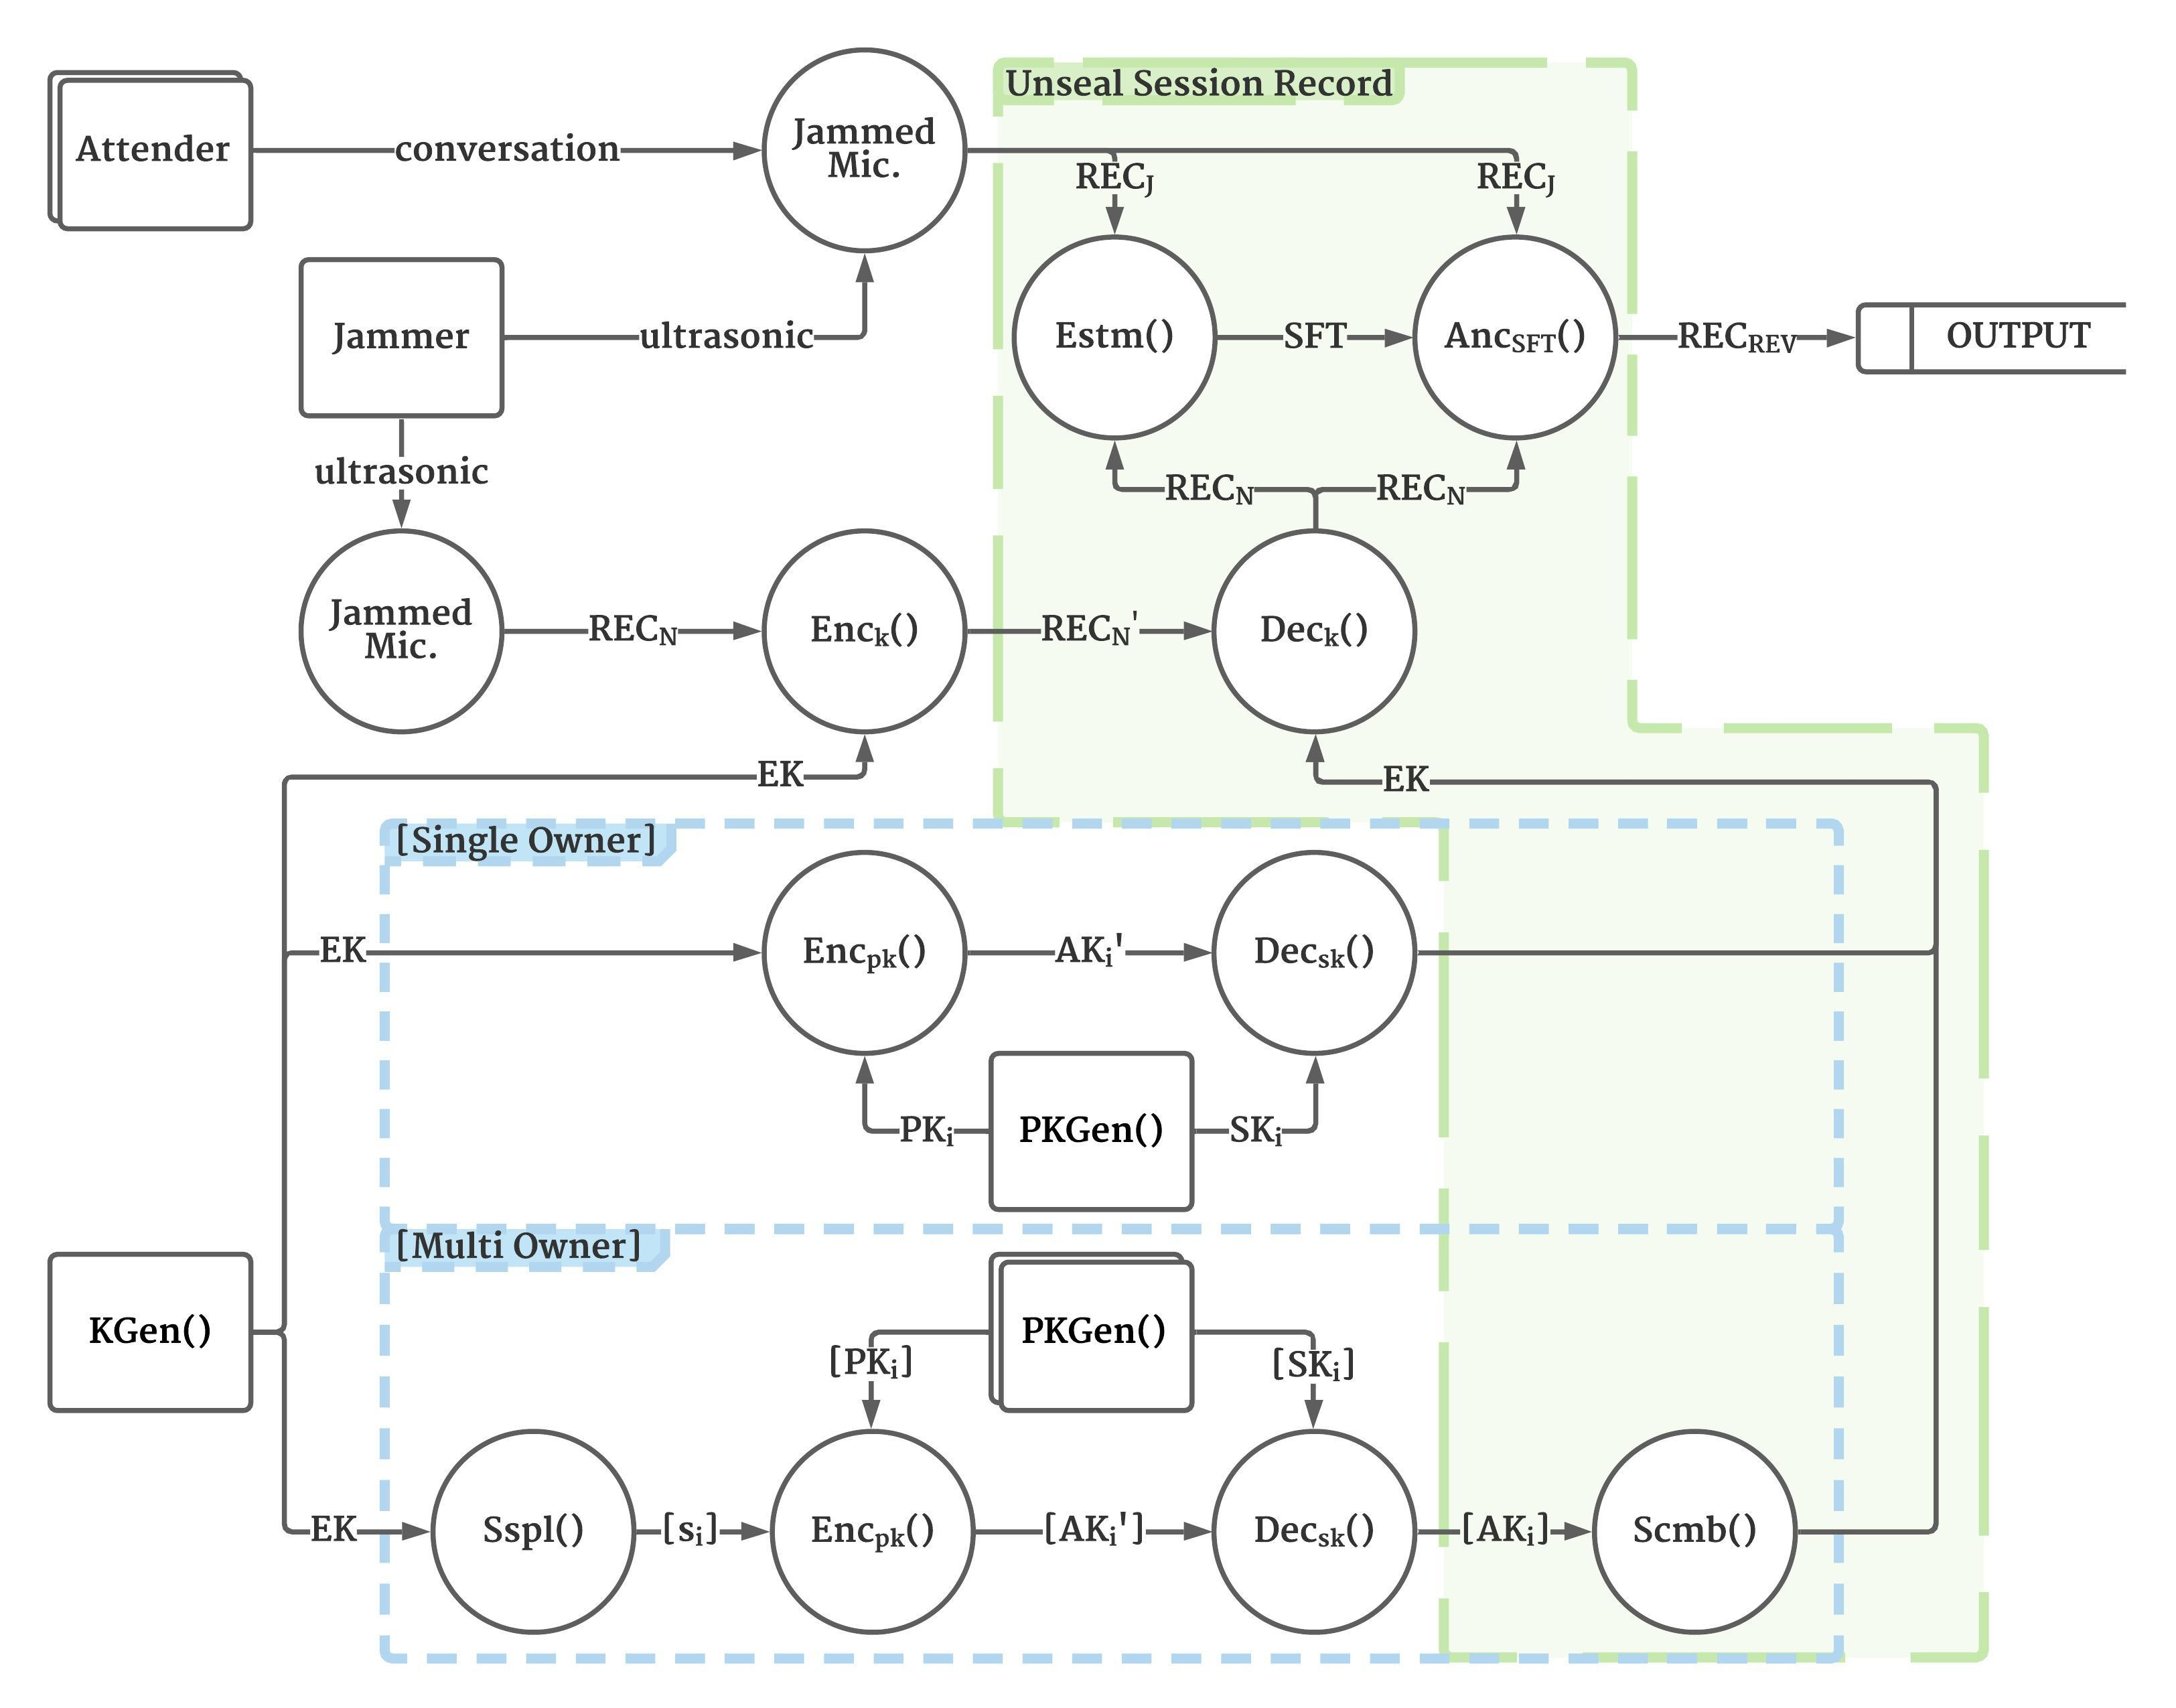
\includegraphics[width=1.0\textwidth]{system-data-flow}
    \caption{系統資料流程圖}\label{fig:system-data-flow}
\end{figure}